\documentclass{article}
\title{AG1 - Cvičení II}
\author{Tommy Chu}
\date{}

\usepackage[czech]{babel}
\usepackage[utf8]{inputenc}
\usepackage[T1]{fontenc}
\usepackage{graphicx}
\usepackage{amsmath}
\usepackage{amsthm}
\usepackage{amssymb}
\usepackage{subfiles}
\usepackage{hyperref}
\usepackage{geometry}
\usepackage{mathtools}
\usepackage{algpseudocode}
\usepackage{algorithm}
\usepackage{physics}
\usepackage{dsfont}
\usepackage{bm}
\usepackage{bbm}
\usepackage{float}
\usepackage{enumitem}
\usepackage{graphicx}
\usepackage{multirow}
\usepackage{tikz}
\usepackage{tikz-cd}
\usepackage{pgfplots}
\usepackage{lmodern}
\usepackage{import}
\usepackage{microtype}
\usepackage{fancyhdr}
\usepackage{parskip}
\usepackage{mystyle}
\usepackage{xcolor}
\usepackage{soul}

\newcommand{\mathcolorbox}[2]{\colorbox{#1}{$\displaystyle #2$}}
\definecolor{grey}{rgb}{.93,.93,.93}

\begin{document}
\maketitle

\section*{Zadání 1}

Formulujte nutné (a rozumné) podmínky pro fakt, že jsou dva grafy $G$, $H$ isomorfní. \\
Formálně: pro dva grafy $G$, $H$ definujte formuli $\varphi(G, H)$ tak, aby platilo tvrzení: \[ G \cong H \implies \varphi(G, H) \]

\subsection*{Řešení}

Nechť jsou grafy $G$ a $H$ isomorfní a funkce $f \colon V(G) \rightarrow V(H)$ isomorfismus těchto grafů. Dále nechť jsou $u, v$ libovolné vrcholy na $G$. Pak platí následující formule:
\begin{align*}
    \varphi_1(G, H) \overset{def}{\iff} & \lvert V(G) \rvert = \lvert V(H) \rvert                                                  \\
    \varphi_2(G, H) \overset{def}{\iff} & \lvert E(G) \rvert = \lvert E(H) \rvert                                                  \\
    \varphi_3(G, H) \overset{def}{\iff} & \exists (\text{$u$-$v$-cesta v $G$}) \implies \exists (\text{$f(u)$-$f(v)$-cesta v $H$}) \\
    \varphi_4(G, H) \overset{def}{\iff} & \text{$G$ a $H$ mají stejný počet souvislých komponent}                                  \\
    \varphi_5(G, H) \overset{def}{\iff} & \text{existuje matice sousednosti reprezentující současně $G$ a $H$}                     \\
\end{align*}
Intuice za formulemi: Po odmyslení labelů vrcholů jsou $G$ a $H$ identické grafy.

\newpage
\section*{Zadání 2}

Nutné podmínky z minulého zadání formálně dokažte z definice isomofismu.

\subsection*{Řešení}

Dokážu formule $\varphi_1$ a $\varphi_3$.
\textbf{Důkaz formule $\varphi_1$:}

\[
    \varphi_1(G, H) \overset{def}{\iff} \lvert V(G) \rvert = \lvert V(H) \rvert
\]

Z předpokladu existuje bijekce $f \colon V(G) \rightarrow V(H)$, pro kterou nutně platí $\lvert D_f \rvert = \lvert H_f \lvert$ -- vlastnost bijektivního zobrazení:
\[
    |V(G)| = |D_f| = |H_f| = |V(H)|
\]
\qed

\textbf{Důkaz formule $\varphi_3$:}

\[
    \varphi_3(G, H) \overset{def}{\iff} \exists (\text{$u$-$v$-cesta v $G$}) \implies \exists (\text{$f(u)$-$f(v)$-cesta v $H$}) \\
\]
Uvažujme libovolnou $u$-$v$-cestu v $G$:
\[u = g_1, \{g_1, g_2\}, g_2, \cdots, g_{n} = v \]
kde $g_i \in V(G)$ pro $i \in \{1, ..., n\}$. Protože se jedná o cestu, jistě platí $g_i \ne g_j$ pro různé indexy $i, j \in \{1, ..., n\}$.

Označme $h_i \coloneqq f(g_i)$ pro $i \in \{1, ..., n\}$: Díky isomorfismu a existující $g_1$-$g_n$-cestě v $G$, přímo odvodíme i existenci $h_1$-$h_n$-cesty v $H$:
\begin{alignat*}{13}
            & f(g_1), &  & \{f(g_1), f(g_2)\}, &  & f(g_2), &  & \cdots, &  & f(g_{n}) \\
    = \quad & h_1,    &  & \{h_1, h_2\},       &  & h_2,    &  & \cdots, &  & h_{n}
\end{alignat*}
kde lze nahradit $h_1 = f(g_1) = f(u)$ a $h_n = f(g_n) = f(v)$. Skutečně se jedná o $f(u)$-$f(v)$-cestu v $H$: Na $H$ platí $f(g_i) \ne f(g_j)$ pro různé indexy $i, j \in \{1, ..., n\}$, protože $f$ je injektivní a na stejných indexech platí $g_i \ne g_j$.
\qed

\newpage
\section*{Zadání 3}

Ukažte, že následující dvě podmínky jsou ekvivalentní pro číslo $n \in \mathbb{N}, n \ge 1$:
\begin{enumerate}
    \item Existuje samodoplňkový graf na $n$ vrcholech.
    \item $n \equiv 1 \pmod{4}$ nebo $n \equiv 0 \pmod{4}$
\end{enumerate}

\subsection*{Řešení}

$1. \implies 2.$:
Samodoplňkový graf $G$ na $n$ vrcholech má jistě stejný počet hran jako svůj doplněk:
\[
    G \cong \overline{G}
    \implies \lvert E(G) \rvert = \lvert E(\overline{G}) \rvert
\]
Dále víme, že velikost sjednocení hran grafu $G$ a jeho doplňku $\overline{G}$ je $\binom{n}{2}$. Počet hran grafu $G$ je proto polovina z počtu všech možných hran v grafu na $n$ vrcholech $\binom{n}{2}/2$.
\begin{align*}
             & \lvert E(G) \rvert + \lvert E(\overline{G}) \rvert = \binom{n}{2}
    \implies 2 \lvert E(G) \rvert = \binom{n}{2}                                 \\
    \implies & \lvert E(G) \rvert = \frac{\binom{n}{2}}{2}
    = \frac{\frac{n!}{(n-2)! 2!}}{2}
    = \frac{\frac{n(n-1)}{2}}{2}
    = \frac{n(n-1)}{4}
\end{align*}

Počet hran v grafu musí být celočíselné, proto $\frac{n(n-1)}{4}$ musí být celé číslo. To platí pouze tehdy, když je $n(n-1)$ dělitelné $4$:
\begin{align*}
    n(n-1) \equiv 0 \pmod{4})
\end{align*}
Součin dvou po sobě jdoucích kladných čísel (sudé $\cdot$ liché) je dělitelné číslem 4 jen, pokud je jeden z činitelů ($n$ nebo $n-1$) násobkem 4:
\begin{align*}
     & n \equiv 0 \pmod{4} \quad \lor \quad n - 1 \equiv 0 \pmod{4} \\
    \Longleftrightarrow \quad
     & n \equiv 0 \pmod{4} \quad \lor \quad n \equiv 1 \pmod{4}
\end{align*}
\qed

$2. \implies 1.$:

Pro jednoduchost zpočátku uvažujme pouze $n \equiv 0 \pmod{4}$, respektive $n \in \{ 4k \mid k \in \mathbb{N} \}$.

Nechť jsou čtyři neprázdné množiny vrcholů $A_1, A_2, B_1, B_2$, $|A_1|=|A_2|=|B_1|=|B_2|=\frac{n}{4}$. Tvrdím, že graf $G$ definován následujícím způsobem je samodoplňkový:
\begin{align*}
    G = ( A_1 \cup A_2 \cup B_1 \cup B_2, \binom{A_1 \cup A_2}{2}
     & \cup \{ \{a_1, b_1\} \mid a_1 \in A_1, b_1 \in B_1 \} \\
     & \cup \{ \{a_2, b_2\} \mid a_2 \in A_2, b_2 \in B_2 \}
    )
\end{align*}
Podgraf grafu $G$ indukovaný množinou $A_1 \cup A_2$ je úplný a naopak podgraf indukovaný množinou $B_1 \cup B_2$ je tvořen izolovanými vrcholy. Odmyslíme-li si hrany mezi vrcholy v $A_1$ a $A_2$, grafy indukované množinou vrcholů $A_1 \cup B_1$ a $A_2 \cup B_2$ jsou úplné `bipartitní' grafy. Pro $n = 8$ může $G$ vypadat následovně:

\begin{center}
    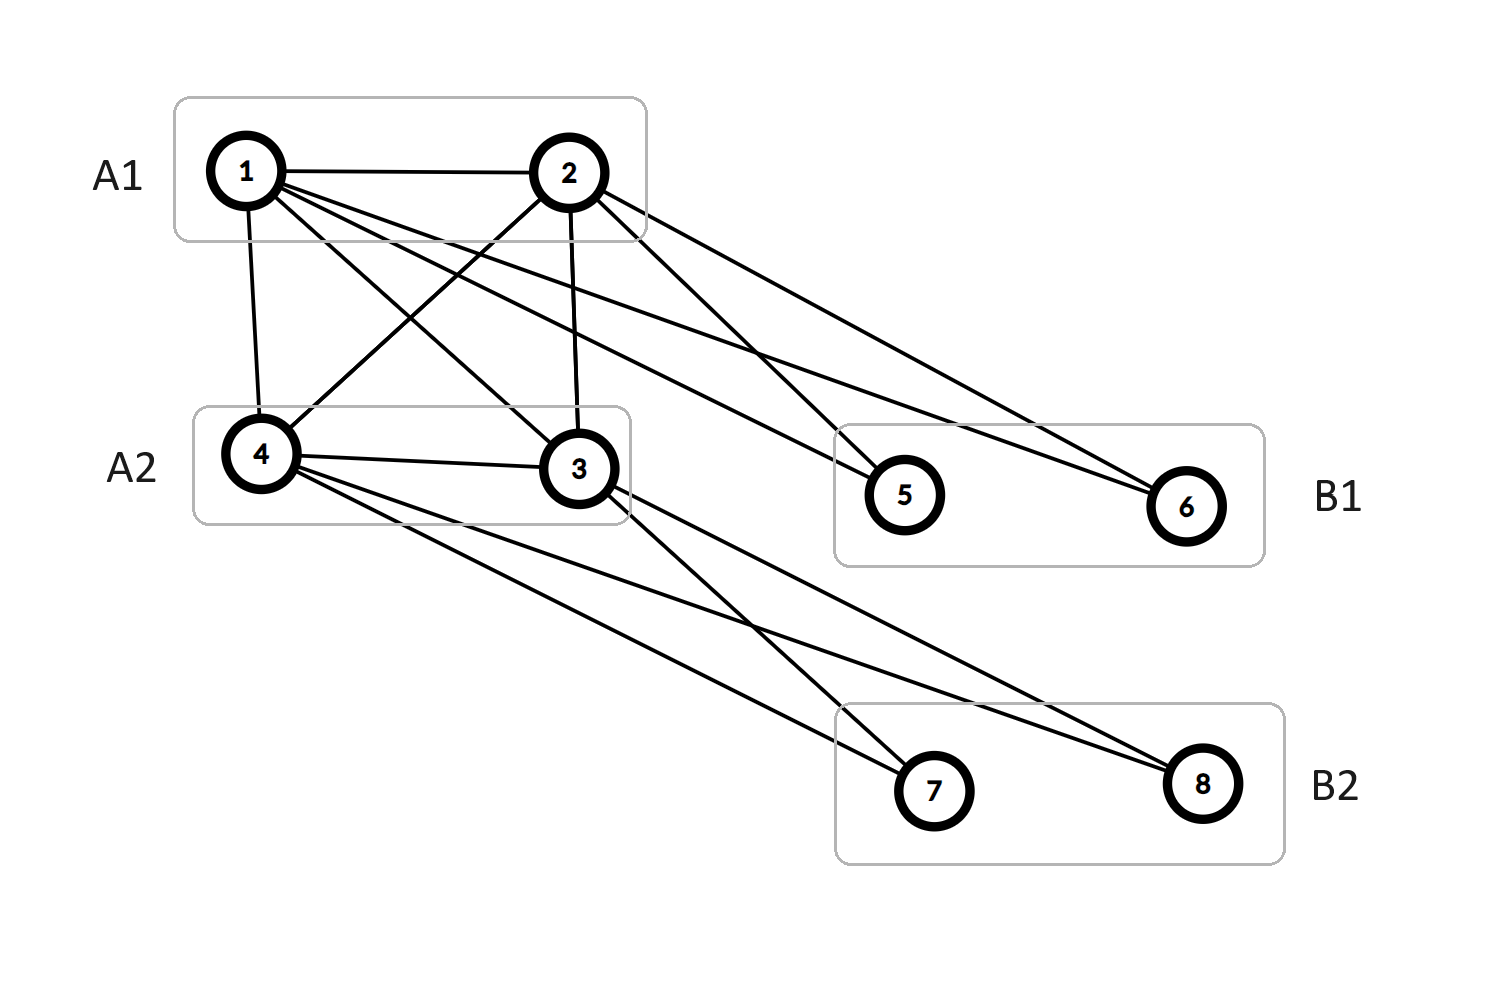
\includegraphics[width=10cm]{before}
\end{center}

Z jistých pozorovní o $G$ lze přímo odvodit vlastnosti o jeho doplňku $\overline{G}$:
\begin{itemize}[parsep=0pt, itemsep=0pt]
    \item[(1a)] mezi všemi vrcholy v $A_1 \cup A_2$ vedou hrany,
    \item[$\xRightarrow{\overline{G}}$] mezi vrcholy v $A_{1} \cup A_{2}$ nevede žádná hrana,
    \item[(1b)] mezi vrcholy v $B_1 \cup B_2$ nevede žádná hrana,
    \item[$\xRightarrow{\overline{G}}$] mezi všemi vrcholy v $B_{1} \cup B_{2}$ vedou hrany,
    \item[(2a)] ze všech vrcholů v $A_1$ vede hrana do každého vrcholu v $B_1$,
    \item[$\xRightarrow{\overline{G}}$] z $A_{1}$ nevede žádná hrana do $B_{1}$,
    \item[(2b)] ze všech vrcholů v $A_2$ vede hrana do každého vrcholu v $B_2$,
    \item[$\xRightarrow{\overline{G}}$] z $A_{2}$ nevede žádná hrana do $B_{2}$,
    \item[(3a)] z $A_1$ nevede žádná hrana do $B_2$,
    \item[$\xRightarrow{\overline{G}}$] ze všech vrcholů v $A_{1}$ vede hrana do každého vrcholu v $B_{2}$,
    \item[(3b)] z $A_2$ nevede žádná hrana do $B_1$,
    \item[$\xRightarrow{\overline{G}}$] ze všech vrcholů v $A_2$ vede hrana do každého vrcholu v $B_{1}$.
\end{itemize}

Z těchto pozorování lze jednoznačně zkonstruovat doplněk grafu $G$:
\begin{align*}
    \overline{G} = ( A_1 \cup A_2 \cup B_1 \cup B_2, \binom{B_1 \cup B_2}{2}
     & \cup \{ \{a_1, b_2\} \mid a_1 \in A_1, b_2 \in B_2 \} \\
     & \cup \{ \{a_2, b_1\} \mid a_2 \in A_2, b_1 \in B_1 \}
    )
\end{align*}

Jedná se o definici grafu $G$ s prohozenými množinami $A_1 \leftrightarrow B_1$ a $A_2 \leftrightarrow B_2$. Protože jsou vrcholy v rámci jedné množiny i samotné celé množiny $A_1, A_2, B_1, B_2$ zaměnitelné, jsou grafy $G, \overline{G}$ isomorfní. Isomorfismus je $f \coloneqq f_1 \cup f_2 \cup f_3 \cup f_4$:
\begin{align*}
     & f_1 : A_{1} \rightarrow B_{1_{\overline{G}}}
     & f_2 : A_{2} \rightarrow B_{2_{\overline{G}}} \\
     & f_3 : B_{1} \rightarrow A_{1_{\overline{G}}}
     & f_4 : B_{2} \rightarrow A_{2_{\overline{G}}} \\
\end{align*}
kde $f_i, i \in \{1, 2, 3, 4\}$ jsou libovolné příslušné bijekce -- libovolné díky zmíněné zaměnitelnosti.

Kdybychom měli v každém případě o jeden vrchol $u$ navíc, v grafu $G$ bychom ho spárovaly se všemi vrcholy v $A_1 \cup A_2$ a v doplňku by nám `přeskočil' na množinu $B_1 \cup B_2$, což by zachovalo symetrii se zbytkem doplňku. Definice by se nám mírně změnily tímto způsobem:
\begin{align*}
    G = ( \colorbox{grey}{\{u\}} \cup A_1 \cup A_2 \cup B_1 \cup B_2, \binom{A_1 \cup A_2}{2}
     & \cup \{ \{a_1, b_1\} \mid a_1 \in A_1, b_1 \in B_1 \}               \\
     & \cup \{ \{a_2, b_2\} \mid a_2 \in A_2, b_2 \in B_2 \}               \\
     & \mathcolorbox{grey}{ \cup \{ \{u, a\} \mid a \in A_1 \cup A_2 \} })
\end{align*}

\begin{align*}
    \overline{G} = ( \colorbox{grey}{\{u\}} \cup A_1 \cup A_2 \cup B_1 \cup B_2, \binom{B_1 \cup B_2}{2}
     & \cup \{ \{a_1, b_2\} \mid a_1 \in A_1, b_2 \in B_2 \}             \\
     & \cup \{ \{a_2, b_1\} \mid a_2 \in A_2, b_1 \in B_1 \}             \\
     & \mathcolorbox{grey}{\cup \{ \{u, b\} \mid b \in B_1 \cup B_2 \}})
\end{align*}

a isomofismus: $f \coloneqq \mathcolorbox{grey}{\{(u, u_{\overline{G}})\}} \cup f_1 \cup f_2 \cup f_3 \cup f_4$. Seznam pozorování by se nám rozšířil:
\begin{itemize}[parsep=0pt, itemsep=0pt]
    \item[(4a)] z vrcholu $u$ vede hrana do každého vrcholu v $A_1 \cup A_2$
    \item[$\xRightarrow{\overline{G}}$] mezi vrcholem $u$ a $A_{1} \cup A_{2}$ nevede žádná hrana,
    \item[(4b)] mezi vrcholem $u$ a $B_1 \cup B_2$ nevede žádná hrana,
    \item[$\xRightarrow{\overline{G}}$] z vrcholu $u$ vede hrana do každého vrcholu v $B_{1} \cup B_{2}$.
\end{itemize}

Analogicky platí již odiskutovaná symetrie a $G, \overline{G}$ jsou isomorfní i pro $n \in \{ 4k + 1 \mid k \in \mathbb{N} \}$.
Ukázali jsme, že pokud $n \equiv 1 \pmod{4}$ nebo $n \equiv 0 \pmod{4}$, existuje samodoplňkový graf na $n$ vrcholech.
\qed

\end{document}